\documentclass[pdftex,12pt,a4paper]{report}

\usepackage[portuguese,english]{babel}
\usepackage[T1]{fontenc} 
\usepackage[utf8]{inputenc}
\usepackage[pdftex]{graphicx}
\usepackage{minitoc}
\usepackage{hyperref}
\usepackage{indentfirst}
\usepackage[compact]{titlesec}
\usepackage{fancyhdr}
\usepackage{caption}
\usepackage{pgfplots}
\usepackage{pgfplotstable}
\usepackage{fixltx2e}
\usepackage{mathtools}
\usepackage{fancyhdr}
\usepackage{listings}
\usepackage{color}
\usepackage{sverb}
\usepackage[section]{placeins}

%Highlight
\newcommand{\shellcmd}[1]{\indent\indent\texttt{\footnotesize\# #1}\\}

\pagestyle{fancy}
\renewcommand*\thesection{\thechapter\arabic{section}}
\newcommand{\HRule}{\rule{\linewidth}{0.5mm}}
\begin{document}

\begin{titlepage}

\begin{center}


\includegraphics[width=0.15\textwidth]{./logo}\\[0.5cm]    

\textsc{\large Universidade de Aveiro \\[1cm]\large departamento de electrónica, telecomunicações e informática}\\[1cm]

\textsc{\large{42566}\large - Arquitectura de Redes Avançadas \\[1cm]}

\HRule \\[0.5cm]
{ \huge \bfseries 2015 Project}\\[0.4cm]
{ \large \bfseries Engineer responsible for the network of ISP X}\\[0.4cm]
\HRule \\[1cm]

\textsc{\small{8240 - MESTRADO INTEGRADO EM ENGENHARIA DE COMPUTADORES E TELEMÁTICA}}\\[1cm]

\begin{minipage}{0.4\textwidth}

\begin{flushleft} \large
\href{mailto:rafael.ferreira@ua.pt}{António Rafael da \\ Costa Ferreira }
 \small{\\NMec: 67405}
\end{flushleft}
\end{minipage}
\begin{minipage}{0.4\textwidth}

\begin{flushright} \large
\href{mailto:rodrigocunha@ua.pt}{Rodrigo Lopes \\ da Cunha}
\small{\\NMec: 67800}
\end{flushright}
\end{minipage}\\[1cm]

{\large Docente: Paulo Salvador }\\[0.5cm]

\vfill

{\large Janeiro de 2016 \\ 2015-2016}

\end{center}

\end{titlepage} %Titulo do Relatorio
\renewcommand{\headrulewidth}{0pt}

%Cabeçalhos de rodapé
\fancyhead{}
\fancyfoot{}
\lhead{Engineer responsible for the network of ISP X}
\rhead{ARA - 2015/2016}
\lfoot{Rafael Ferreira nmec: 67405 \\ Rodrigo Cunha nmec: 67800}
\rfoot{\thepage}

%Renomear Comandos
\renewcommand*\contentsname{Conteúdos}
\renewcommand*\figurename{Figura}
\renewcommand*\tablename{Tabela}

%Conteúdos, dar paragrafo
\tableofcontents
%Headers
\renewcommand{\headrulewidth}{0.15pt}
\renewcommand{\thechapter}{}

\clearpage

\section{Introdução}
% o que, porquê e o objetivo
O trabalho proposto para o projeto da unidade curricular de Arquitectura Avançada de Redes é assumir o papel de um engenheiro de redes responsável por um ISP X com o sistema autónomo AS 9.345.
Estas relações serão estabelecidas pelos routers em Lisboa e no Porto.  O ISP X será um não transito ISP, ou seja, anuncia apenas rotas locais.
O ISP tem dois clientes, a empresa A e a empresa B, que será responsável por lhes dar conectividade para a Internet e será responsável pelo serviço VOIP com conectividade PSTN. Também terá um servidor DNS condicional e uma Firewall.
A empresa A tem duas branches, uma em Aveiro e outra em Faro, a conectividade é dada usando o Router EmpA1 e o Router EmpA2.
A empresa B tem apenas uma localização em Aveiro, no entanto, a empresa B é um sistema autónomo privado.
O ISP S dá conectividade para o PSTN através do SIP Proxy 2. O ISP L dá conectividade para o Internet Core.
O relatório reflete todos os passos e decisões tomadas.

\clearpage

\section{Visão Geral}

\begin{figure}[!htb]
\center
 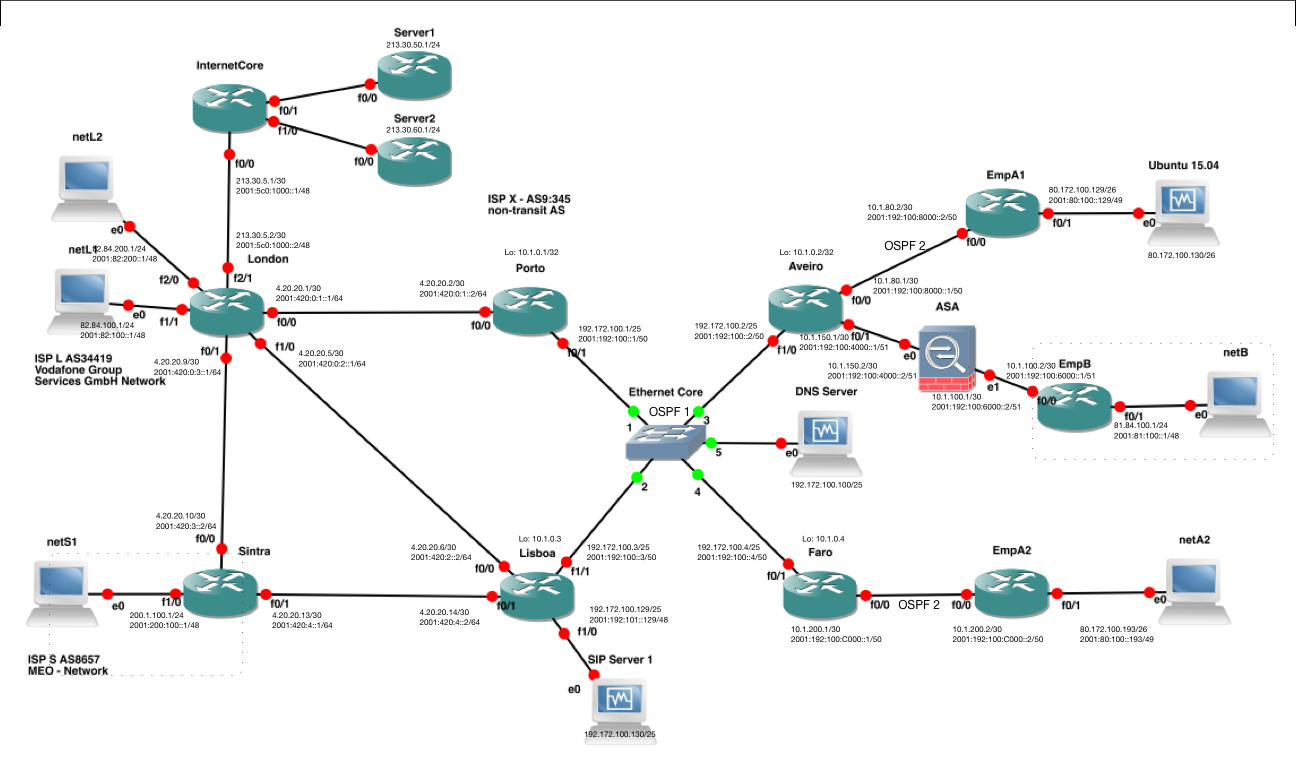
\includegraphics[width=150mm,scale=1]{imagens/mapa.png}
 \caption{Mapa de IP's}
 \label{fig:mapadeips}
\end{figure}

A divisão dos IPs foi feita tendo em conta o quadro que nos foi dado no enunciado.

\begin{figure}[!htb]
\center
 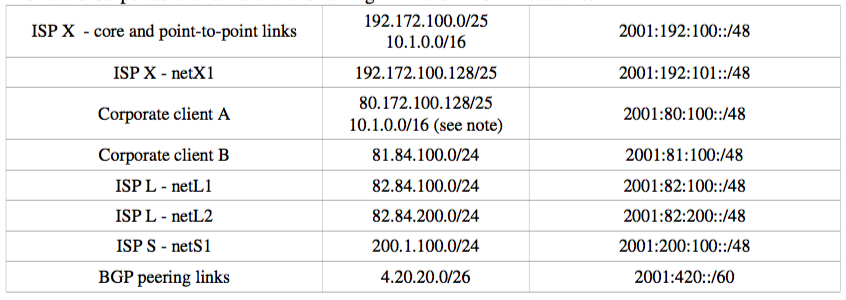
\includegraphics[width=150mm,scale=1]{imagens/devisaodeips.png}
 \caption{IPv4 e IPv6}
 \label{fig:mapadeips}
\end{figure}

\newpage

\section{Conectividade IPv4}

\subsection{Relação do ISP X com os outros ISPs}

A relação entre o ISP X e os seus ISPs vizinhos é feita tendo em conta o que foi pedido, algo importante é que não fosse um ISP de trânsito, ou seja, apenas anuncia rotas locais para os seus ISPs vizinhos. No entanto, foi tido em atenção para não anunciar redes privadas para os seus vizinhos e para que a rede do sistema autónomo da empresa B seja anunciada para estes. Outra coisa que se teve em atenção foi anunciar a rede da empresa A como um agregado.

\begin{figure}[!htb]
\center
 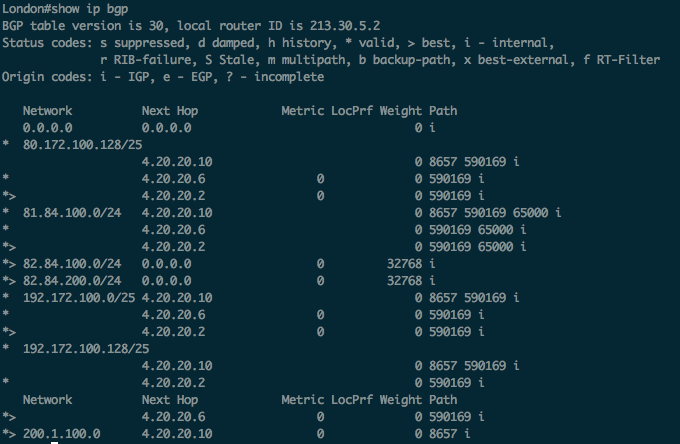
\includegraphics[width=65mm,scale=1]{imagens/showipbgp_london.png}
 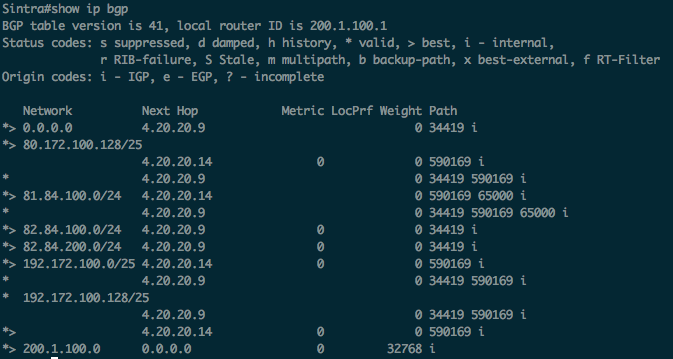
\includegraphics[width=65mm,scale=1]{imagens/showipbgp_sintra.png}
 \caption{Londres e Sintra}
 \label{fig:mapadeips}
\end{figure}

Como se pode observar na figura anterior, Sintra apenas conhece as redes que é suposto conhecer. Não conhece redes privadas do ISP X e conhece a rede da Empresa B. A rede da empresa A é anunciada como um agregado. Também conhece as redes de Londres.

\newpage

\subsection{Empresa B}

\begin{figure}[!htb]
\center
 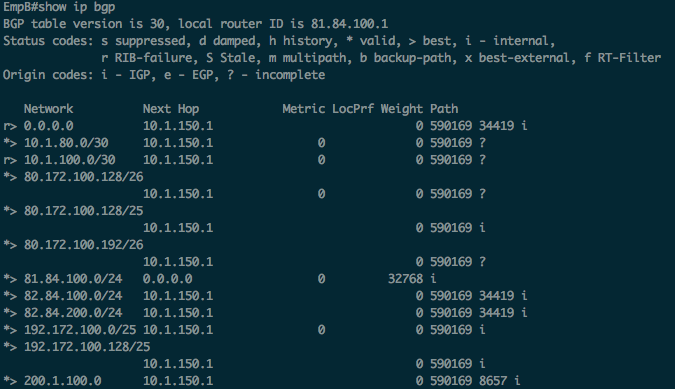
\includegraphics[width=65mm,scale=1]{imagens/showipbgp_empb.png}
 \caption{Sintra}
 \label{fig:mapadeips}
\end{figure}

A empresa B conhece as redes de Londres por BGP, as do ISP X e as anunciadas por Sintra.

\subsection{Routing Constraints}

De forma a que Aveiro e Faro consigam fazer a preferência local para determinadas rotas é necessário que Porto e Lisboa façam a marcação das rotas quando as recebem. 

Para isso, Porto deve marcar as redes netL1 e netL2 para enviar como uma community para Aveiro. Assim Aveiro ao receber essa comunidade irá aumentar a preferência para as rotas recebidas com essa comunidade. Porque Aveiro deve ter como preferência Porto para ir para as redes netL1 e netL2.

Já Lisboa deve marcar também as redes netL1 e netL2 com outra comunidade para enviar para Aveiro e Faro, assim Faro ao receber essa comunidade irá também aumentar a preferência para essas rotas recebidas, porque Faro deve enviar parar a netL1 e netL2 preferencialmente por Lisboa.

Já para o tráfego ser roteado para a Internet preferencialmente via Lisboa (ISP S), todas as rotas externas devem ser anunciadas  com uma community para Aveiro e Faro para serem marcadas como preferência o seu roteamento por Lisboa. Mas isso não chega, é preciso que em Lisboa também haja preferência a ser enviado pelo ISP S.

Para o tráfego IP para a rede netS1 ser apenas roteado via Lisboa usando a ligação direta para o ISP S é necessário que em Lisboa apenas aceite esta rede por Sintra e no Porto não a aceite por Londres.

\subsection{OSPF e BGP}

Existe um processo OSPF a correr no internet core e outro para a Empresa A que tem o intuito de ser usado redistribuindo para a VPN entre a EmpA1 e a EmpA2. As relações BGP são estabelecidas usando os IPs das interfaces Loopback.

\section{MPLS}

\subsection{MPLS tunnels for SIP traffic com uma reserva de 1Mbps}
Os túneis que são necessários para a reserva de 1Mbps é entre Aveiro >< Lisboa e entre Faro >< Lisboa para dar reserva de largura de banda para a empresa A e para empresa B para o tráfego SIP, entre Aveiro e Lisboa serão 2 túneis e entre Faro e Lisboa outro túnel.

O tráfego de SIP é encaminhado para dentro do tunnel usando uma ip policy na interface que diz respeito a este tipo de tráfego.

\subsection{MPLS VPN para a Empresa A, ligando Aveiro e Faro}
Para a VPN da empresa A que liga Aveiro e Faro foi usado uma vrf para o efeito que tem um processo OSPF para ser mais fácil a distribuição das rotas dentro da VRF. Fora da VRF foram criadas rotas estáticas para dar a conhecer as redes públicas que devem ser conhecidas dentro do ISP X. Para chegar à Internet foi usado uma rota estática para enviar para a routing table global pedidos que na VRF sejam para a rota default.

\section{VoIP - SIP}

Foi criado um servidor SIP na netX1, denominado de Servidor SIP Proxy 1. Este é responsável por dar conectividade VoIP entre clientes e fazer reencaminhamento das chamadas mesmo que sejam números não atribuidos. O forwarding deve ser feito para o SIP Proxy 2.

\section{CDN}

Foi criado um servidor para Conditional DNS para servir os clientes do ISP. Foram seguidos os mesmos passos do guia que está no elearning para o efeito.

\section{Firewall}

A firewall criada entre Aveiro e a Empresa B teve de ter alguns cuidados, teve de se ter cuidado em deixar passar tráfego para o BGP e tráfego para ICMP tanto para IPv4 para IPv6.

\newpage

\section{Conclusão}

O principal objetivo foi conseguido, queria-se fazer os 22 valores do trabalho para termos uma noção minimalista do que um Operador normalmente tem de ter e as várias possibilidades que podem ser feitas e soluções que podem ser desenvolvidas. 

Este trabalho serviu para meter em prática muita coisa que tinha sido falado na teórica e que ainda não se tinha tido oportunidade de se meter em prática num só, sendo assim, o projeto foi divertido e interessante de ser realizado.

\end{document}